\documentclass[12pt, a4paper, oneside]{ctexart}
\usepackage{amsmath, amsthm, amssymb, appendix, bm, graphicx, hyperref, mathrsfs}

\CTEXsetup[format={\Large\bfseries}]{section}

\title{\textbf{测试报告}}
\author{第25组}
\date{\today}

\begin{document}

\maketitle

\section{概述}
本次测试执行了所有的测试计划。总的覆盖率结果如下图所示,没有达到100\%是因为有一部分代码本身是不可能执行到的。

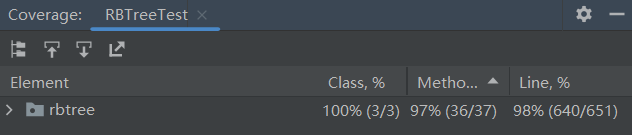
\includegraphics[scale=0.5]{screenshots/coverage.png}

下面列出对于每个方法的单元测试的测试结果和覆盖率分析。

\section{对search方法的测试}

\subsection{测试结果}
通过了所有的测试用例。

\subsection{覆盖率分析}
执行tree.search(6)时,控制流经过的路径为 J A B D E G I K

执行tree.search(5)时,控制流经过的路径为 J A B D E F A B D E G H A B D E G I K

执行tree.search(114514)时,控制流经过的路径为 J A B D E G H A B D E G H A B C K

因此,三条路径覆盖了三个变量x, key, cmp的定义节点到所有使用节点以及后续节点的定义-清除路径。
根据全使用准则,覆盖率为100\%。

\section{对minimum方法的测试}

\subsection{测试结果}
通过了所有的测试用例。

\subsection{覆盖率分析}
调用第一个tree.minimum()时,控制流经过的路径为 A B C

调用第二个tree.minimum()时,控制流经过的路径为 A B D E F E G

因此,两条路径覆盖了变量this.mRoot和p的定义节点到所有使用节点以及后续节点的定义-清除路径。
根据全使用准则,覆盖率为100\%。

\section{对maximum方法的测试}

\subsection{测试结果}
通过了所有的测试用例。

\subsection{覆盖率分析}
调用第一个tree.maximum()时,控制流经过的路径为 A B C

调用第二个tree.maximum()时,控制流经过的路径为 A B D E F E G

因此,两条路径覆盖了变量this.mRoot和p的定义节点到所有使用节点以及后续节点的定义-清除路径。
根据全使用准则,覆盖率为100\%。

\section{对leftRotate方法的测试}

\subsection{测试结果}
通过了所有的测试用例。

\subsection{覆盖率分析}
从上到下三次leftRotate的控制流分别为:

A B C D E F J

A B D E G H J

A B D E G I J

满足$C_1p$指标,覆盖率为100\%。

\section{对rightRotate方法的测试}

\subsection{测试结果}
通过了所有的测试用例。

\subsection{覆盖率分析}
从上到下三次rightRotate的控制流分别为:

A B C D E F J

A B D E G H J

A B D E G I J

满足$C_1p$指标,覆盖率为100\%。

\section{对insertFixUp方法的测试}
\subsection{测试结果}
    通过了所有的测试用例。

\subsection{覆盖率分析}
    从上到下覆盖了所有\textbf{可达}的DD路径。

\section{对insert方法的测试}
\subsection{测试结果}
    通过了所有的测试用例。

\subsection{覆盖率分析}
    从上到下覆盖了所有\textbf{可达}的DD路径。

\section{对removeFixUp方法的测试}
\subsection{测试结果}
    通过了所有的测试用例。

\subsection{覆盖率分析}
    代码覆盖率为100\%,满足$C_0$指标。

\section{对remove方法的测试}
\subsection{测试结果}
    通过了所有的测试用例。

\subsection{覆盖率分析}
    代码覆盖率为100\%,满足$C_0$指标。

\section{各小组成员贡献比例}
谭博仁、周峰和张贻天贡献均为33\%,KENT HUGO GEMIARTHA贡献为0。

\end{document}